% encoding: utf8
% !TEX encoding = utf8
% !TeX spellcheck = pl_PL

\newpage\hspace{0cm}\thispagestyle{empty}
\newpage\thispagestyle{empty}
\noindent
\begin{tabular}{p{4.3cm} p{11cm}}
	\noindent
	%%% Zdjęcie
	\begin{minipage}{4.5cm}
		\center
		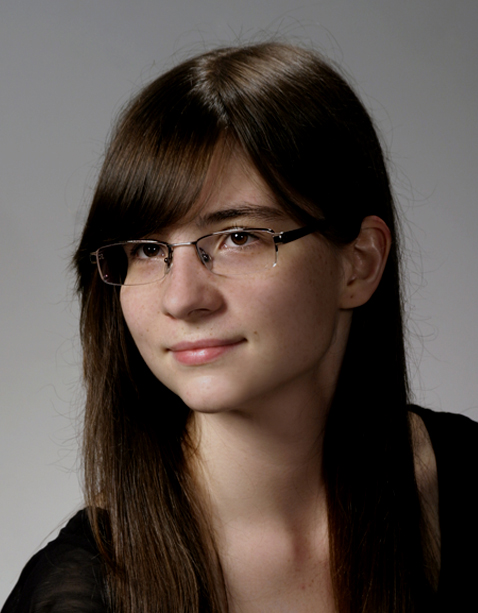
\includegraphics[height=5.5cm]{images/poczatek/photo.jpg}
	\end{minipage}
	&
	%%% Data urodzenia, specjalność itp.
	\begin{minipage}{9.7cm}
		Kierunek: \hfill Informatyka \\[5mm]
		Specjalność: \hfill Inżynieria Systemów Informatycznych\\[5mm]
		Data rozpoczęcia studiów: \hfill 2015\\
	\end{minipage}
\end{tabular}
% \vspace*{0.2\baselineskip}
%%%%%%%%%%%%%%%%%%%%%%%%%%%%%%%%%%%%%%%%%%%%%%%%%%%%%%%%%%%%%%%%%%%%%%%%%%%%%%%%
%%% Życiorys
%%%%%%%%%%%%%%%%%%%%%%%%%%%%%%%%%%%%%%%%%%%%%%%%%%%%%%%%%%%%%%%%%%%%%%%%%%%%%%%%
\begin{center}
	{\large\bfseries Życiorys}\par %\bigskip
\end{center}

% TODO

\par
\vspace{0.2\baselineskip}
\hfill\parbox{15em}{{\small\dotfill}\\[-.3ex]
	\centerline{\footnotesize podpis studenta}}\par

\vspace{1\baselineskip}
\cleardoublepage
% Nowa strona.
\newpage\thispagestyle{empty}

% Podziękowanie
\begin{center}
	\vspace{10mm}
	\vspace{20mm}
	\begin{flushright}
		\begin{tabular}{r}
		\end{tabular}
	\end{flushright}
	\vfill
	\textbf{Podziękowanie}\\
	Dziękuję wszystkim osobom, które w~sposób merytoryczny i~edytorski przyczyniły się do powstania niniejszej pracy. Dziękuję całej załodze KNR ,,Bionik'' za nieocenioną pomoc i~wsparcie.
\end{center}

% Nowa strona.
\newpage\hspace{0cm}\thispagestyle{empty}
\newpage\thispagestyle{empty}
\noindent

